% Two slides: data collection, and graph creation and cleaning.
% To use in the main deck: copy the two frames below, the figures/ folder,
% and the packages marked "needed by the frames" into the main preamble.
\documentclass[aspectratio=169]{beamer}

% needed by the frames
\usepackage{amsmath}
\graphicspath{{figures/}}

\setbeamertemplate{navigation symbols}{}

\begin{document}

% ---------------------------------------------------------------- slide 1
\begin{frame}{Data collection}
\centering
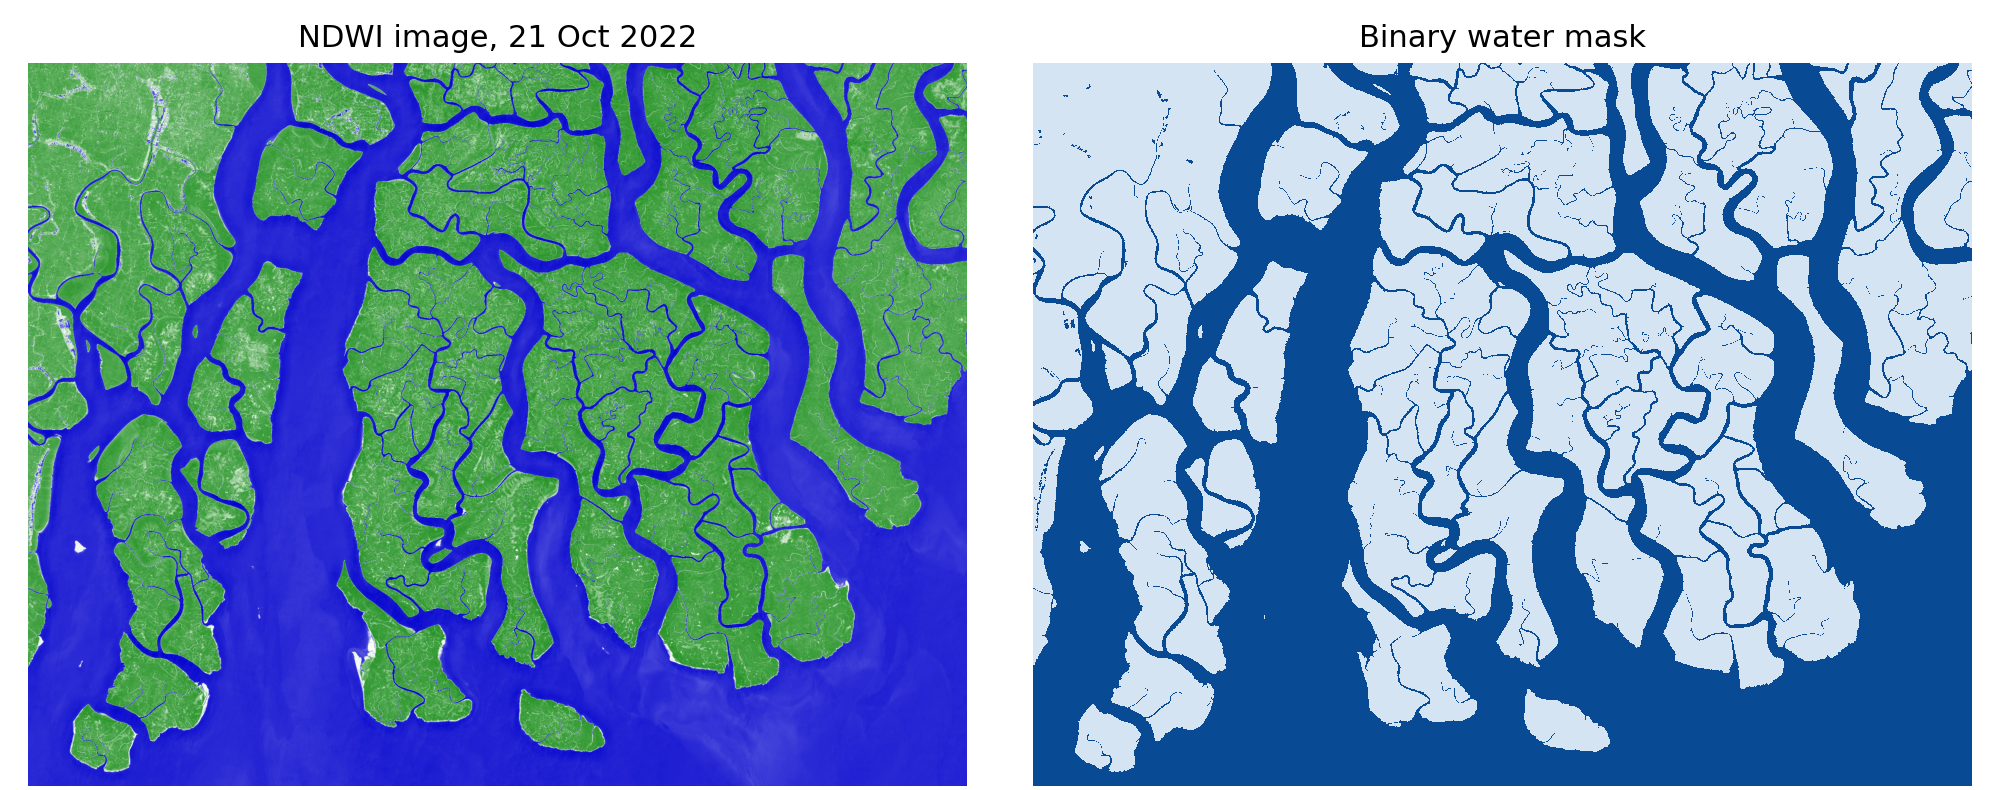
\includegraphics[width=0.70\textwidth]{image_and_mask.png}

\vspace{2mm}
\begin{columns}[T,onlytextwidth]
\begin{column}{0.48\textwidth}
\footnotesize
\begin{itemize}\setlength{\itemsep}{2pt}
  \item Satellite images from the Copernicus Browser
  \item One a year, mid-Oct to mid-Nov, 2016--2026, on low-cloud days
  \item 30 m per pixel: 2500 $\times$ 1925 px $\approx$ 75 $\times$ 57.75 km
\end{itemize}
\end{column}
\begin{column}{0.48\textwidth}
\footnotesize
\textbf{Water index:} \;$\text{NDWI} = \dfrac{\text{Green} - \text{NIR}}{\text{Green} + \text{NIR}}$

\vspace{1mm}
Water absorbs near-infrared (NIR); vegetation and soil reflect it. Near $+1$: deep water; near $-1$: vegetation or land.
\begin{itemize}\setlength{\itemsep}{1pt}
  \item Otsu's threshold: minimises the variance within each class
  \item Objects under 30 px removed
\end{itemize}
\end{column}
\end{columns}
\end{frame}

% ---------------------------------------------------------------- slide 2
\begin{frame}{Graph creation and cleaning}
\centering
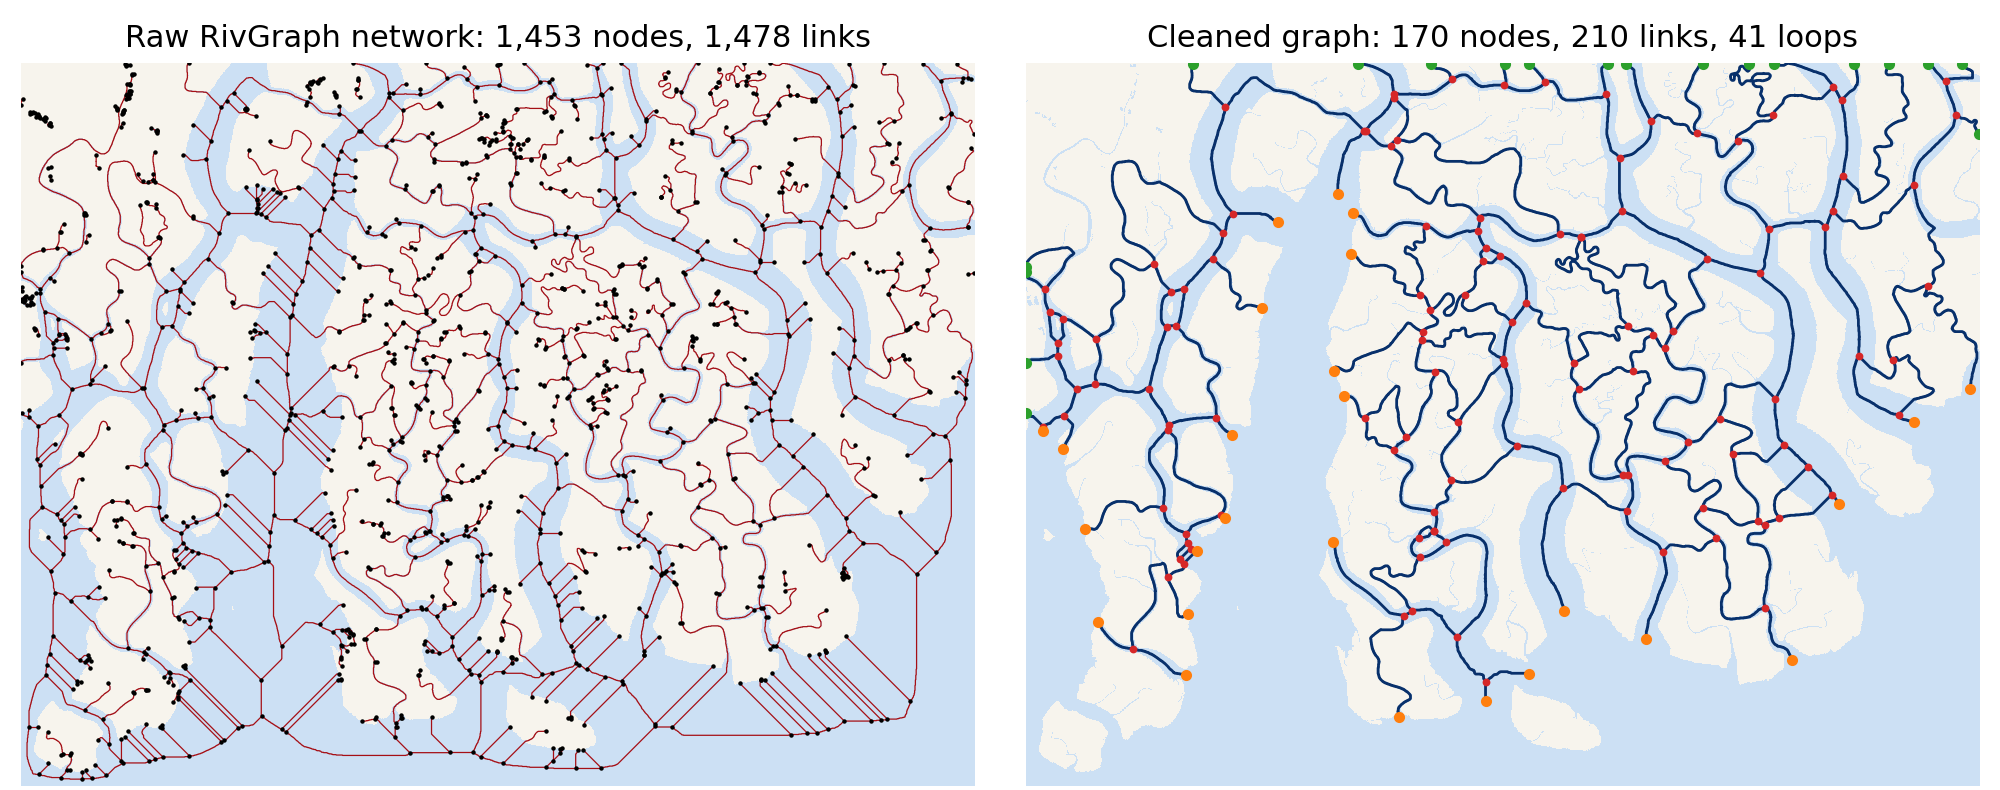
\includegraphics[width=0.70\textwidth]{raw_vs_clean.png}

\vspace{2mm}
\begin{columns}[T,onlytextwidth]
\begin{column}{0.48\textwidth}
\footnotesize
\begin{enumerate}\setlength{\itemsep}{2pt}
  \item Inlets: degree-1 nodes on the top, left or right edge
  \item Shoreline: a polygon boundary around all landmasses
  \item Nodes beyond the shoreline are replaced by outlet nodes, merged into one outlet
\end{enumerate}
\end{column}
\begin{column}{0.48\textwidth}
\footnotesize
\begin{enumerate}\setcounter{enumi}{3}\setlength{\itemsep}{2pt}
  \item Remove degree-1 nodes other than inlets and the outlet
  \item Remove degree-2 nodes and connect their neighbours directly
  \item Keep only the giant component
\end{enumerate}
\end{column}
\end{columns}

\vspace{2mm}
\alert{\small Result: $<$200 nodes, $\sim$30--40 loops; degree 1 or 3, plus the single outlet.}
\end{frame}

\end{document}
